% !TEX root = main_min_disc_dist.tex
\subsection{Double Integrator}
The doube integrator consists of two states $(x_1, x_2)$ , and  control $u \in [u_{min}, u_{max}]$ with dynamics,
\begin{equation}
\begin{split}
\dot{x_1} & = x_2 \\
\dot{x_2} & = u 
\end{split}
\end{equation}
In our experiments, we discretize the state space, to a $161 \times 161$ grid.

We first show, in Fig~\ref{fig:convergence} that $Z$ over approximates~(bold line) and under approximates~(dotted lines) the true reachable set~(shown in black) for two values of $\lambda = 0.1, 0.2$. The target set $\mathcal{T}$ is shown in red. 
\begin{figure}
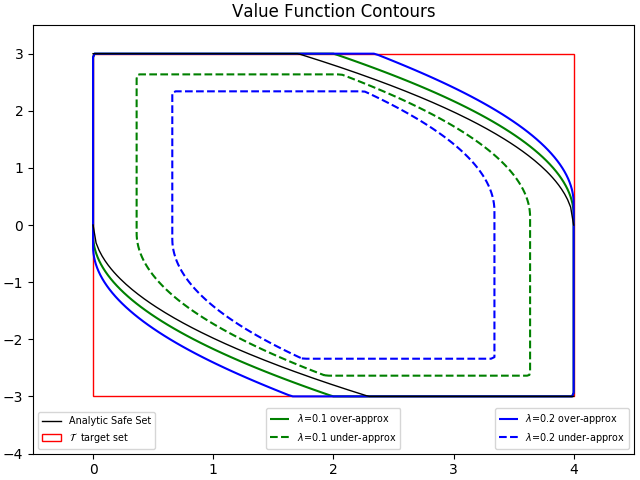
\includegraphics[scale=0.5]{convergence_difflambda.png}
\caption{The analytic reachable set $V$ and target set $\mathcal{T}$ are shown in black and red. The over and under approximated $Z_{\lambda}$ are shown in bold green and dotted green for $\lambda=0.1$; and bold blue and dotted blue line for $\lambda  = 0.2$. This suggests smaller the value of $\lambda$, the better $Z_{\lambda}$ approximates $V$.}
\label{fig:convergence}
\end{figure}

We next compare value iteration and policy iteration with increasing number of discrete actions in Table~\ref{tab:v_vs_p}. In the table we see that as the number of actions increase, there is sharp increase in how long value iteration takes to converge while the increase is much smaller for policy iteration. However, the total time taken for policy iteration is much larger since there is a significant overhead cost in constructing $P_{\pi_u}$ building the matrices for value functions. 
\begin{table}
\centering
\caption{Value Iteration vs Policy Iteration}
\label{tab:v_vs_p}
\begin{tabular}{|c| c| c| c|}
\hline
\# actions & VI & \multicolumn{2}{|c|}{Policy Iteration} \\ \cline{3-4}
 &  $T_{total} (Iters)$ & $T_{total}(Iters)$ & $T_{total} - T_{P_{\pi_u}}$ \\ \hline
2 & 1.255 (204) & 68.793 (4) & 0.105 \\ \hline
50 &  7.562 (204)&  69.717 (4)& 0.365 \\ \hline
250 & 32.841 (204)&  251.39 (14)& 3.504 \\ \hline
500 & 63.815 (204)&  253.855 (14)& 6.741 \\
\hline
\end{tabular}
\end{table}

Finally, we ran value iteration from different initializations, the signed distance function $Z_0 = l(\cdot)$ and an all zeros $Z_0= 0$. The converged values functions had a norm of $0.000299$ between them, suggesting that MDR converges independent of the initialization. However, running MR with $V_0 = 0$, does not converge to the true value function.